O método de Descida máxima, ou método do gradiente, se baseia em um método muito simples para encontrar o mínimo de uma função.
 A partir de um ponto inicial calcula-se a direção de maior de crescimento, de descida máxima ou sentido inverso do gradiente, que dão nome ao método, 
e faz-se um avanço nessa mesma direção.\\
 
Como sabemos, o gradiente de uma função representa sua direção de maior crescimento. Sabendo disso utiliza-se a direção oposta, 
mas a questão que fica é qual o avanço é necessário. Para resolver isso, a direção do gradiente foi normalizada, $d^k$, e criou-se uma variável, $\alpha$, que indica o avanço a ser feito. 

Com o gradiente calculado naquele ponto, usa-se um método de minimização unidimensional qualquer para minimizar a função $x^k - \alpha d^k$. 
Foi escolhido o método da seção áurea, devido a sua grande flexibilidade e por encontrar o mínimo com poucas iterações e baixo esforço computacional. 
Após a minimização utilizamos o valor de $\alpha$ que a minimiza como avanço.
\\
Dessa forma faz-se a iteração para encontrar o próximo ponto, que a princípio 
está mais perto do mínimo. E assim faz-se até convergir ao ponto de mínimo da função (considerando que a mesma o possui).

Como métodos de parada foram escolhidos o tamanho da norma do vetor diferença de gradiente em cada iteração, a norma entre a diferença entre os pontos em cada iteração e finalmente o número de iterações.

Para verificar a convergência do método vemos como são as direções de avanço do algoritmo e também sua norma. Sabe-se a partir de \cite{Notastioafel} que cada iteração tem direção perpendicular a anterior e que a convergência dá-se quando cada avanço é menor que o anterior, assim como vemos na figura \ref{fig:stegradeszigzag}


\begin{figure}[H]
	\begin{center}
		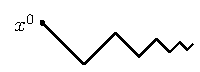
\includegraphics[width=8cm]{../tikz/stegrades}  
		\caption{Representação do avanço convergente em zig-zag com ângulos retos.}
		\label{fig:stegradeszigzag}
	\end{center}
\end{figure}


	\begin{quote}
		\centering
		Lei de Iteração:
	\end{quote}

\begin{equation}
	x^{k+1} = x^k - \alpha d^k
	\end{equation}
	
Após construir o algoritmo, foram feitos testes usando algumas funções:

\begin{itemize}
	\item $ f_1(x,y) = x^2 + y^2$
	\item $ f_2(x,y) = -e^{-x^2 -y^2}$
	\item $ f_3(x,y) = cos(\frac{xy}{5})+sin(\frac{xy}{5}) $
	\item $ f_4(x,y) = |x+y| $
\end{itemize}


\newpage

\begin{figure}[H]
	\begin{center}	
		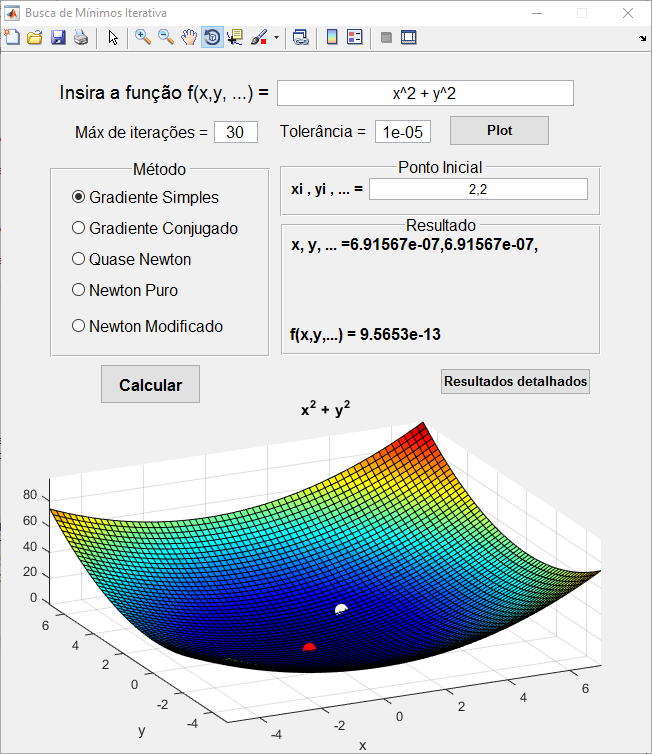
\includegraphics[width=12cm]{../stegrades/f1_gui.PNG}
		\caption{Janela de inicialização de $ f_1(x,y) $}
		\label{fig:f1_gui}
	\end{center}
\end{figure}



\begin{figure}[H]
	\begin{center}	
		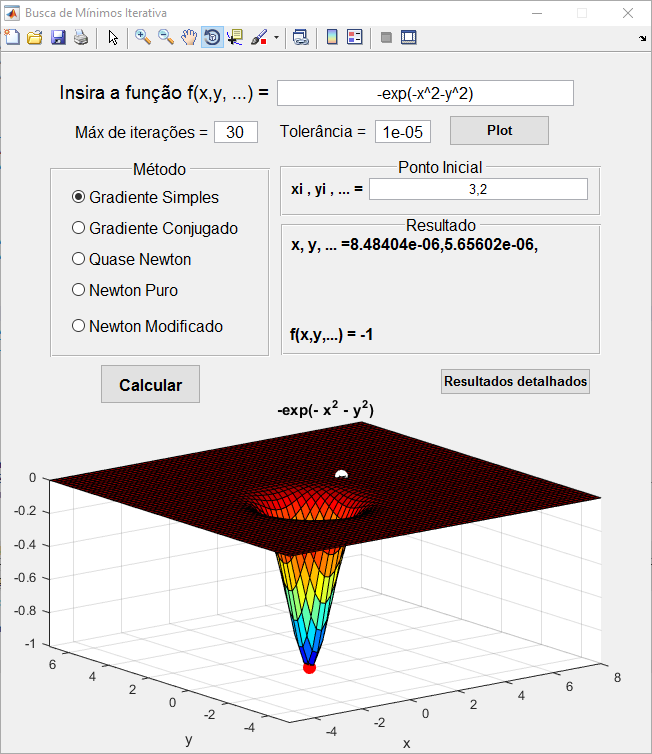
\includegraphics[width=12cm]{../stegrades/f2_gui.PNG}
		\caption{Janela de inicialização de $ f_2(x,y) $}
		\label{fig:f2_gui}
	\end{center}
\end{figure}



\begin{figure}[H]
	\begin{center}	
		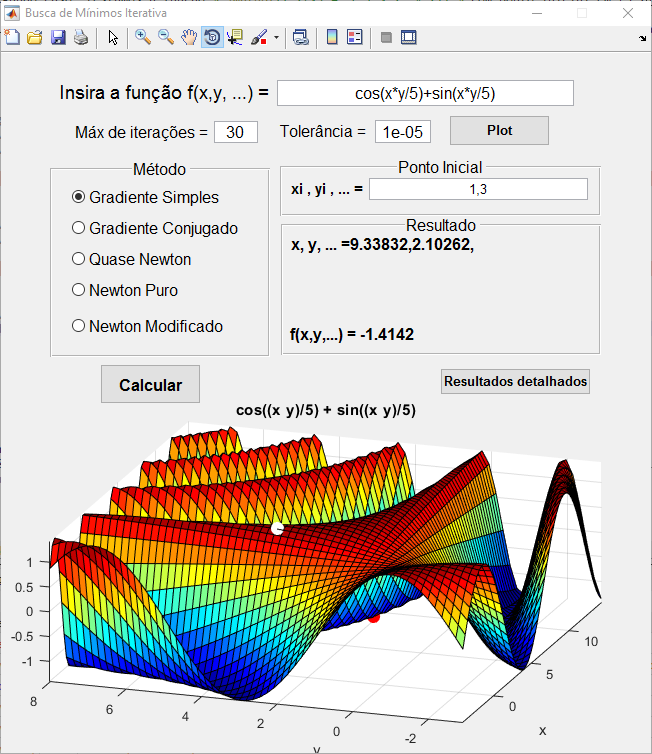
\includegraphics[width=12cm]{../stegrades/f3_gui.PNG}
		\caption{Janela de inicialização de $ f_3(x,y) $}
		\label{fig:f3_gui}
	\end{center}
\end{figure}



\begin{figure}[H]
	\begin{center}	
		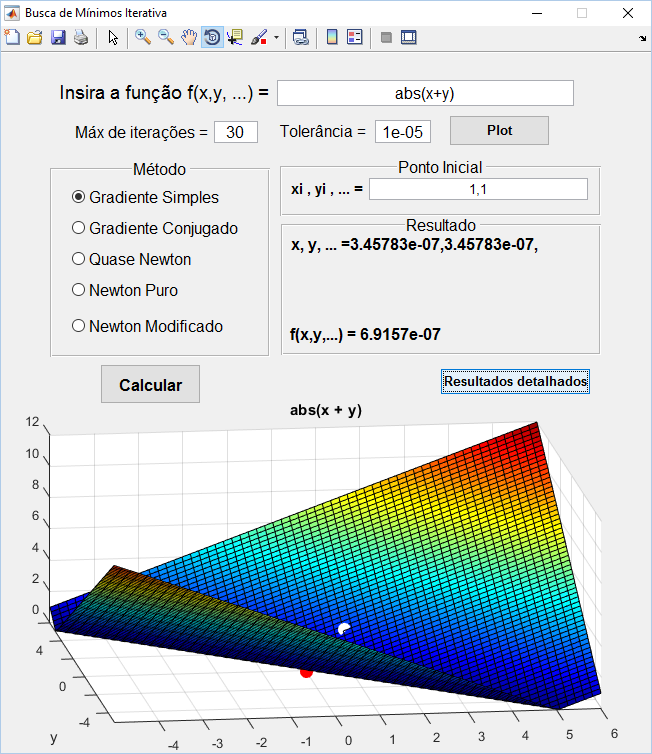
\includegraphics[width=12cm]{../stegrades/f4_gui.PNG}
		\caption{Janela de inicialização de $ f_4(x,y) $}
		\label{fig:f4_gui}
	\end{center}
\end{figure}






\newpage



